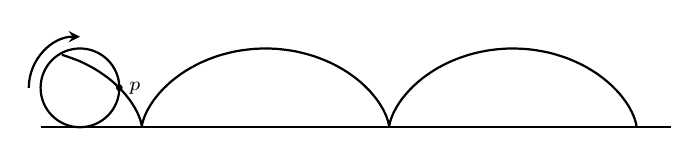
\begin{tikzpicture}[>=stealth,scale=.5]
%\begin{axis}[width=\marginparwidth+25pt,%
%tick label style={font=\scriptsize},axis y line=none,axis x line=none,name=myplot,%
			%%x=.37\marginparwidth,
			%%y=.37\marginparwidth,
			%%xtick={-6,-4,-2,2,4,6},
			%%minor x tick num=4,% 
%%			extra x ticks={.33},
%%			extra x tick labels={$1/3$},
			%%ytick={-3,-2,-1,1,2,3},
			%%minor y tick num=4,%extra y ticks={-5,-3,...,7},%
			%ymin=-4.1,ymax=4.1,%
			%xmin=-4.9,xmax=4.9%
%]
%
%
%\addplot [thick,{\colorone}, smooth,domain=0:360] ({cos(x)},{sin(x)});
%
%
%
%\end{axis}




\draw [thick] (0,1) circle (1);
\filldraw (1,1) circle (2pt) node [right] {\scriptsize $p$};

\draw [{\colorone},thick,domain=-1:14,smooth,samples=60] plot ({cos(\x r)+\x},{-sin(\x r)+1});
\draw [thick] (-1,0) -- (15,0);
%\draw [thick,->] (-.75,2.5) -- (.75,2.5);
\draw [thick,->] (-1.3,1) arc (180:90:1.3);
\draw [thick,white] (0,2.5) -- (1,2.5);
%\node [right] at (myplot.right of origin) {\scriptsize $x$};
%\node [above] at (myplot.above origin) {\scriptsize $y$};
\end{tikzpicture}





















